\documentclass[convert]{standalone}

\usepackage{tikz}
\usepackage{graphicx}
\pagestyle{empty}

% INT_AY22_L23_Fig02_Realistic_Hohmann.png

\begin{document}

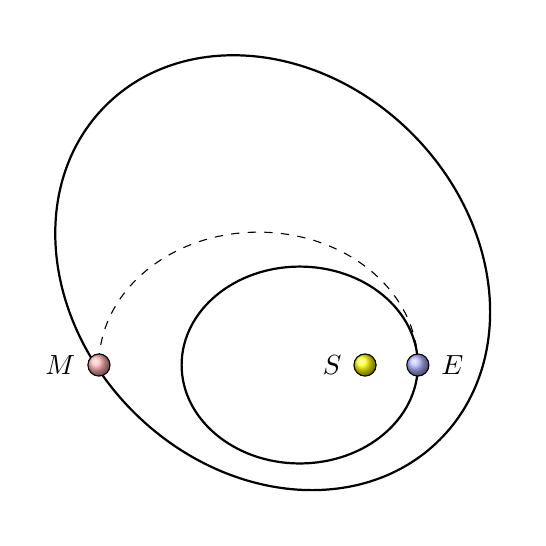
\begin{tikzpicture}[> = latex]

	% Definitions
	
	\def\a{1.5} 		% (Semi-)major axis
	\def\b{1.25} 	% (Semi-)minor axis
	\def\Q{-45}		% Mars orbit relative rotation
	\def\s{2} 		% Ratio of planetary semi-major axes
	\def\sorb{1.35} 	% Ratio of transfer orbit to Earth orbit
	
	% Calculate linear eccentricity
	
	\pgfmathparse{sqrt(\a^2 - \b^2)}
	\let\c\pgfmathresult
	
	% Calculate necessary shift to put Sun
	% at focus of Mars orbit
	
	\pgfmathparse{\c * (1 - \s * cos(\Q))}
	\let\sx\pgfmathresult
	
	\pgfmathparse{-\s * \c * sin(\Q)}
	\let\sy\pgfmathresult

	% Earth orbit
	
	\draw [thick] (0, 0) circle [x radius = \a, y radius = \b];
	
	% Mars orbit

	\draw [thick, xshift = \sx cm, yshift = \sy cm, rotate = \Q] (0, 0) circle [x radius = \s * \a, y radius = \s * \b];
	
	% Hohmann transfer orbit
	
	\draw [dashed] (\a, 0) arc [start angle = 0, end angle = 180, x radius = {\sorb * \a}, y radius = {\sorb * \b}];
	
	% Place planets E and M
	
	\draw [ball color = blue!30] (\a, 0) circle (4 pt) node [right = 0.5 em] {$E$};
	\draw [ball color = red!30] ({\a * (1 - 2 * \sorb)}, 0) circle (4 pt) node [ left = 0.5 em] {$M$};
%	\draw [ball color = red!30] ({\s * \a * cos(180 + \Q) + \sx}, {\s * \a * sin(180 + \Q) + \sy}) circle (4 pt) node [above left = 0.25 em] {$M$};
		
	% Place the Sun S at the right-hand focus; use the
	% linear eccentricity for the x coordinate
	
	\draw [ball color = yellow] (\c, 0) circle (4 pt) node [left = 0.5 em] {$S$};
	
\end{tikzpicture}
\end{document}